\documentclass{article}
\usepackage{graphicx} % new way of doing eps files
\usepackage{listings} % nice code layout
\usepackage[usenames]{color} % color
\usepackage{float}
\definecolor{listinggray}{gray}{0.9}
\definecolor{graphgray}{gray}{0.7}
\definecolor{ans}{rgb}{1,0,0}
\definecolor{blue}{rgb}{0,0,1}
% \Verilog{title}{label}{file}
\newcommand{\Verilog}[3]{
  \lstset{language=Verilog}
  \lstset{backgroundcolor=\color{listinggray},rulecolor=\color{blue}}
  \lstset{linewidth=\textwidth}
  \lstset{commentstyle=\textit, stringstyle=\upshape,showspaces=false}
  \lstset{frame=tb}
  \lstinputlisting[caption={#1},label={#2}]{#3}
}


\author{Jiasen Zhou, Jon Johnston}
\title{Lab 10: Memory}

\begin{document}
\maketitle

\section{Executive Summary}
The purpose of this lab is to design and simulate the Memory stage of the datapath with the iMemory module. The primary functionality of this stage is to manage the data memory used in the load and store commands. However, the branch resolution logic gates are also a part of this stage, and they handle what values are passed to the pc\_src for conditional and unconditional branching. After running the testbench simulation, it is clear that the lab was successful.

\section{Test Report}
To verify operation of these module, this lab requires one test bench. 
\begin{enumerate}
	\item iMemory Test Bench
\end{enumerate}



\pagebreak

\begin{figure}[H]
	\begin{center}
		\caption{Timing diagram for the iMemory test.}\label{fig:iMemorytest}
		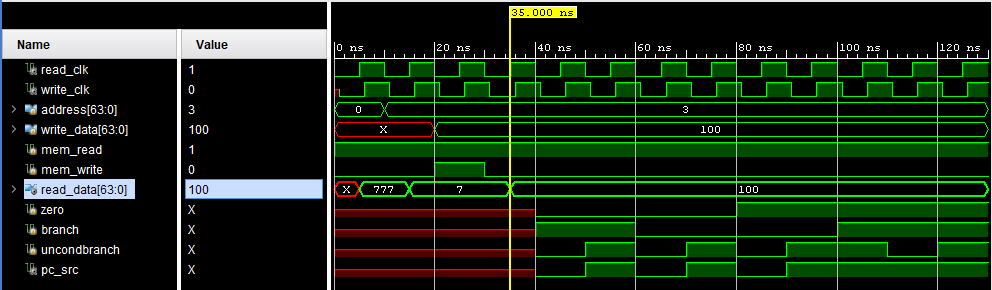
\includegraphics[width=1.0\textwidth]{../images/iMemory_test_timing_diagram.PNG}
	\end{center}
\end{figure}


\section{Code Appendix}
\Verilog{Verilog code for iMemory module.}{code:iMem}{../code/4_Memory/iMemory.v}
\Verilog{Verilog code for data\_mem component.}{code:datamem}{../code/4_Memory/data_mem.v}
\Verilog{Verilog code for testing the iMemory module .}{code:iMemtest}{../code/4_Memory/iMemory_test.v}
\end{document} 